\documentclass[12pt,a4paper]{article}

\usepackage[utf8]{inputenc}
\usepackage[T1]{fontenc}
\usepackage[french]{babel}
\usepackage{lmodern}
\usepackage{geometry}
\usepackage{booktabs}
\usepackage{amsmath}
\usepackage{array}
\usepackage{graphicx}
\usepackage{xcolor}
\usepackage{hyperref}
\usepackage{float}
\usepackage{enumitem}

\geometry{margin=2.5cm}
\hypersetup{
    colorlinks=true,
    linkcolor=teal,
    urlcolor=teal,
    pdftitle={Analyse nutritionnelle des produits USDA},
    pdfauthor={DALINGUESSAN}
}

\title{\textbf{Analyse nutritionnelle des produits USDA\\avec visualisations intégrées}}
\author{Projet Data Science\\DALINGUESSAN}
\date{20 septembre 2026}

\begin{document}

\begin{titlepage}
    \centering
    \vspace*{2cm}
    {\Large Projet Data Science\par}
    \vspace{1.5cm}
    {\Huge\bfseries Analyse nutritionnelle\\des produits USDA\par}
    \vspace{1.5cm}
    {\large Caractéristiques, associations entre variables et analyse en composantes principales\par}
    \vfill
    {\large DALINGUESSAN\\20 septembre 2026\par}
\end{titlepage}

\tableofcontents
\newpage

\section{Introduction}

Les produits alimentaires présentent des compositions nutritionnelles très variées. L'objectif de ce projet est d'explorer la base nationale de nutriments de l'USDA afin de répondre à trois questions :
\begin{enumerate}[label=\arabic*.]
    \item Quelles sont les principales caractéristiques nutritionnelles des produits ?
    \item Quelles associations existent entre les différentes variables ?
    \item Peut-on résumer les profils nutritionnels avec une analyse en composantes principales (ACP) ?
\end{enumerate}

Ce rapport présente directement les principaux résultats sous forme de graphiques intégrés au document. 

\section{Données et préparation}

\subsection{Description de la base}

Le fichier \texttt{USDA\_National\_Nutrient\_DataBase.xlsx} contient une feuille \texttt{ABBREV}. Elle comprend 8\,790 produits et 53 variables. Chaque ligne correspond à un produit identifié par son nom court et son identifiant USDA. Les variables décrivent notamment l'énergie, les macronutriments, les minéraux, les vitamines, les acides gras et le cholestérol.

Les valeurs nutritionnelles sont généralement exprimées pour 100 g de produit. Les variables de poids de portion et de description textuelle sont conservées pour la description, mais ne sont pas intégrées à l'ACP.

\subsection{Valeurs manquantes}

La base présente des taux de valeurs manquantes différents selon les nutriments. Les variables de vitamines et de caroténoïdes sont moins renseignées que l'énergie et les macronutriments. Pour l'ACP, seules les variables ayant au moins 70\% de valeurs disponibles sont retenues, soit 36 variables.

\begin{figure}[H]
    \centering
    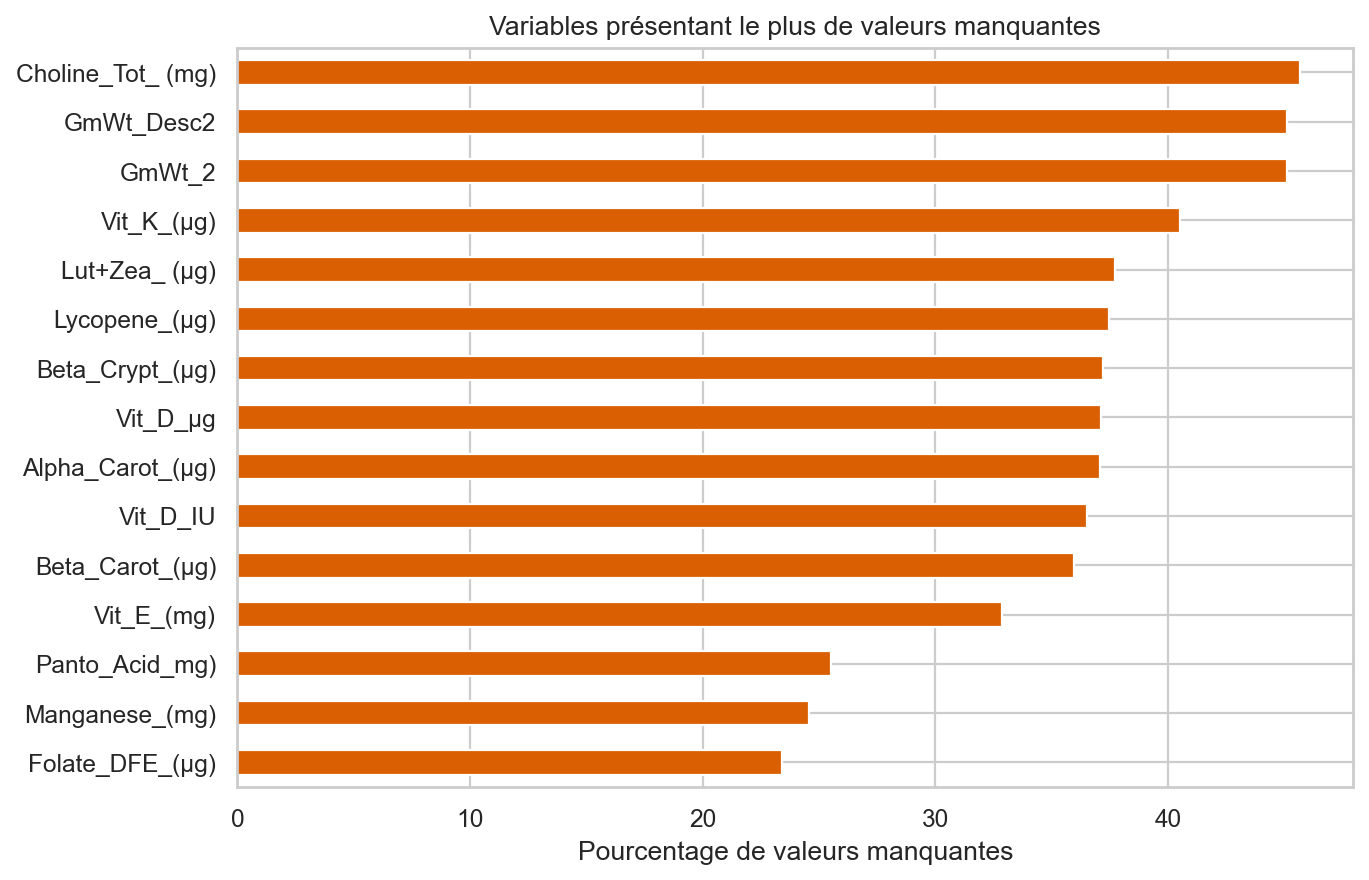
\includegraphics[width=0.82\textwidth]{figures_rapport/valeurs_manquantes.png}
    \caption{Variables présentant le plus de valeurs manquantes.}
    \label{fig:missing}
\end{figure}

Les valeurs manquantes de ces variables sont remplacées par leur médiane. Cette stratégie limite l'influence des valeurs extrêmes et permet de conserver les produits dans l'analyse.

\subsection{Standardisation}

Les unités sont différentes selon les variables : grammes, milligrammes ou microgrammes. Avant l'ACP, chaque variable est donc standardisée selon
\[
    z_{ij}=\frac{x_{ij}-\bar{x}_{j}}{s_j},
\]
où $\bar{x}_{j}$ est la moyenne de la variable $j$ et $s_j$ son écart-type.

\section{Analyse descriptive}

L'analyse descriptive permet de comparer les ordres de grandeur et la dispersion des principaux nutriments. Le tableau suivant résume les variables retenues pour l'interprétation.

\begin{table}[H]
\centering
\caption{Variables nutritionnelles principales}
\label{tab:descriptif}
\begin{tabular}{>{\raggedright\arraybackslash}p{4.2cm}p{7.5cm}}
\toprule
Variable & Interprétation \\
\midrule
\texttt{Energ\_Kcal} & Énergie en kilocalories pour 100 g \\
\texttt{Protein\_(g)} & Protéines en grammes \\
\texttt{Lipid\_Tot\_(g)} & Lipides totaux en grammes \\
\texttt{Carbohydrt\_(g)} & Glucides en grammes \\
\texttt{Fiber\_TD\_(g)} & Fibres alimentaires en grammes \\
\texttt{Sugar\_Tot\_(g)} & Sucres totaux en grammes \\
\texttt{Sodium\_(mg)} & Sodium en milligrammes \\
\texttt{Calcium\_(mg)} & Calcium en milligrammes \\
\bottomrule
\end{tabular}
\end{table}

Les distributions sont hétérogènes et souvent asymétriques. Cette observation justifie la standardisation avant l'ACP. Elle indique également que la moyenne seule ne suffit pas à décrire les produits : la médiane et les quantiles doivent être consultés dans le tableau de bord.

\begin{figure}[H]
    \centering
    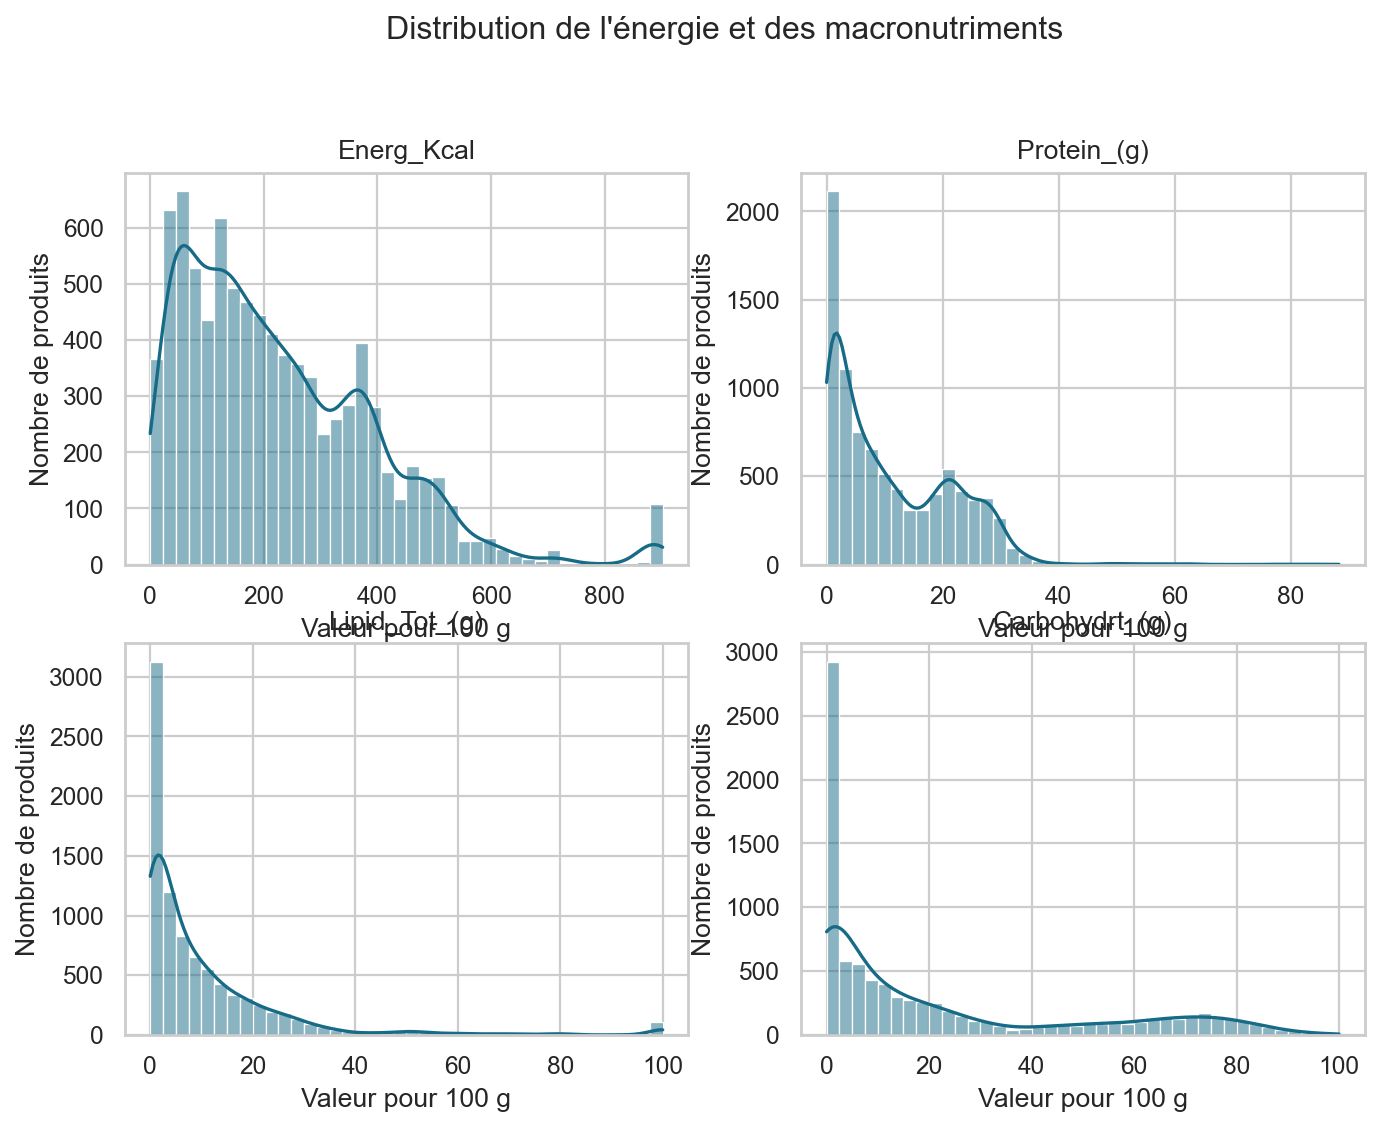
\includegraphics[width=0.92\textwidth]{figures_rapport/distributions.png}
    \caption{Distribution de l'énergie et des principaux macronutriments.}
    \label{fig:distributions}
\end{figure}

\section{Associations entre variables}

Les associations linéaires sont étudiées avec la corrélation de Pearson :
\[
    r_{XY}=\frac{\operatorname{Cov}(X,Y)}{\sigma_X\sigma_Y}.
\]

Une corrélation positive indique que deux variables ont tendance à augmenter ensemble. Une corrélation négative indique qu'une variable augmente lorsque l'autre diminue. Une corrélation ne constitue toutefois pas une preuve de causalité.

Les associations les plus fortes observées sont présentées dans le tableau~\ref{tab:correlations}.

\begin{table}[H]
\centering
\caption{Associations linéaires les plus fortes}
\label{tab:correlations}
\begin{tabular}{lr}
\toprule
Paire de variables & Corrélation \\
\midrule
Vit\_A\_RAE -- Retinol & 0,989 \\
Folate\_Tot -- Folate\_DFE & 0,983 \\
Folic\_Acid -- Folate\_DFE & 0,952 \\
Water -- Energ\_Kcal & -0,901 \\
Lipid\_Tot -- FA\_Mono & 0,885 \\
Folate\_Tot -- Folic\_Acid & 0,880 \\
Vit\_A\_IU -- Vit\_A\_RAE & 0,845 \\
Ash -- Sodium & 0,826 \\
\bottomrule
\end{tabular}
\end{table}

Ces résultats s'expliquent en partie par les relations de définition entre certains indicateurs nutritionnels. Par exemple, plusieurs variables de folates ou de vitamine A mesurent des dimensions proches. La relation négative entre l'eau et l'énergie traduit le fait que les aliments très aqueux sont souvent moins énergétiques pour 100 g.

\begin{figure}[H]
    \centering
    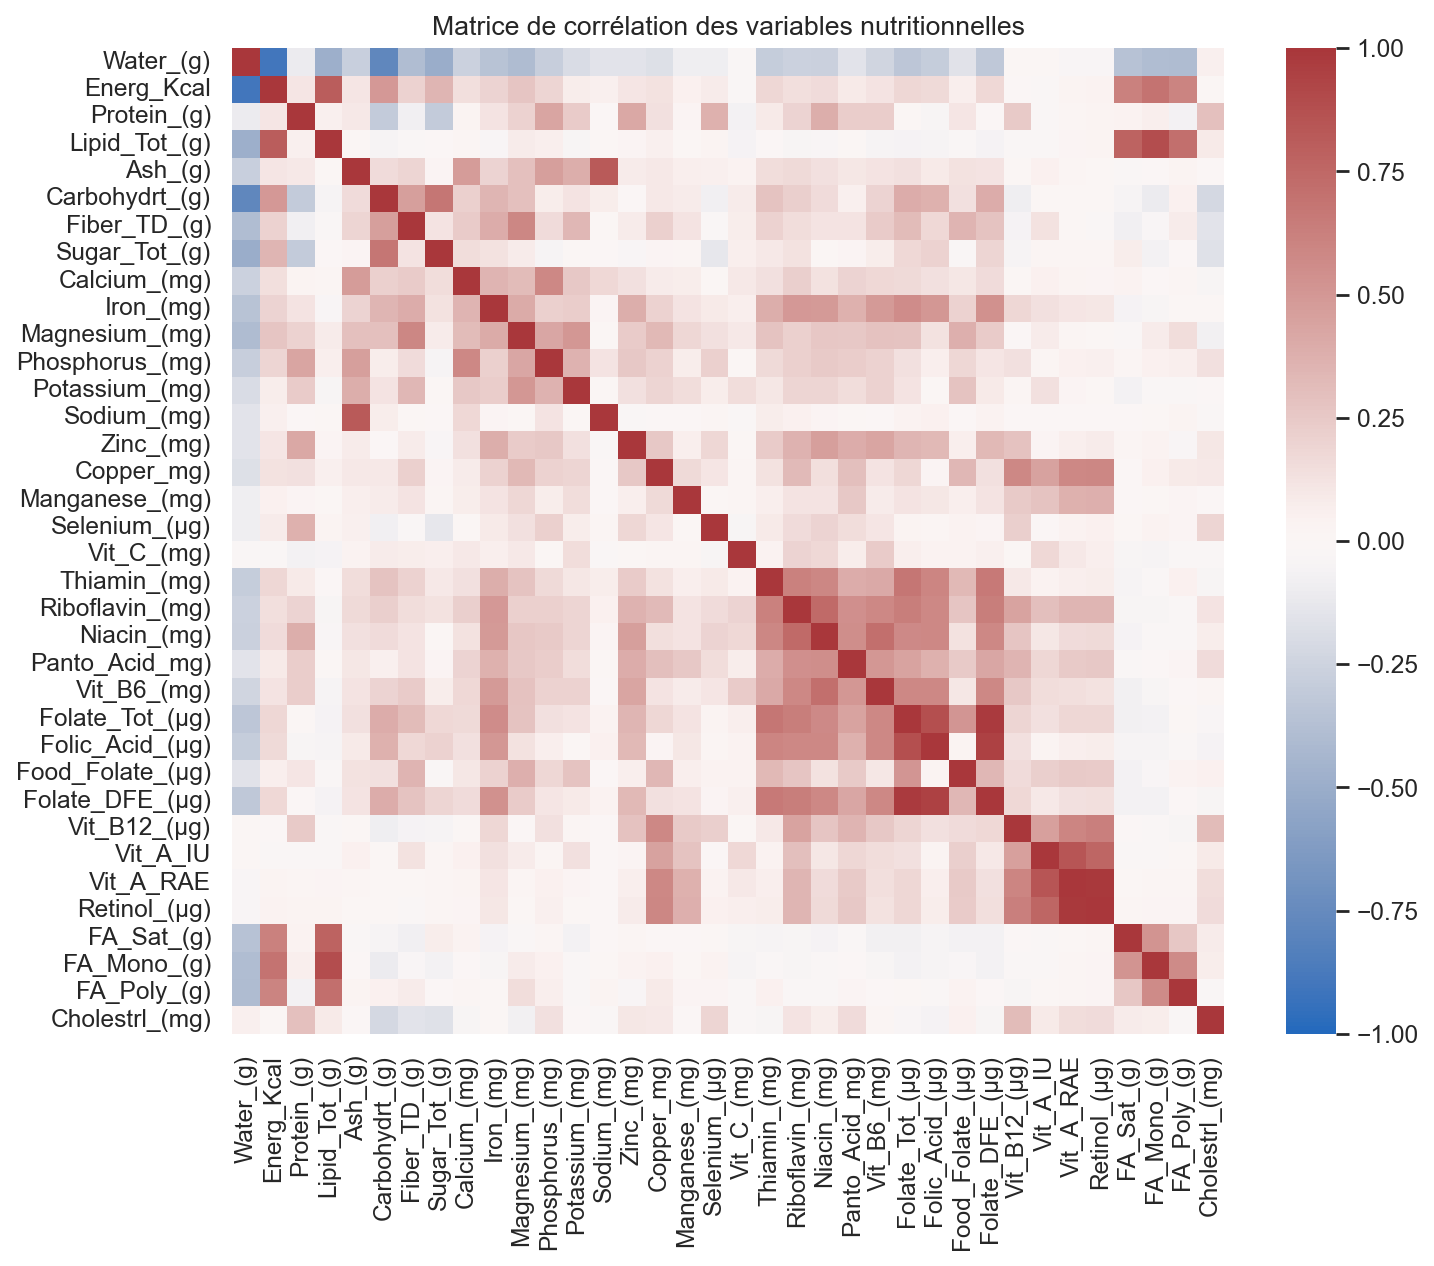
\includegraphics[width=0.88\textwidth]{figures_rapport/correlations.png}
    \caption{Matrice de corrélation des variables nutritionnelles retenues.}
    \label{fig:correlations}
\end{figure}

\section{Analyse en composantes principales}

\subsection{Objectif et méthode}

L'ACP transforme les 36 variables nutritionnelles standardisées en axes non corrélés. Chaque axe est une combinaison linéaire des variables initiales. L'objectif n'est pas de supprimer l'information, mais de la résumer dans un espace de dimension plus faible.

Les deux premiers axes expliquent 32,04\% de la variance totale : le premier axe explique 20,52\% et le deuxième 11,52\%. Ce pourcentage montre que le plan factoriel est utile pour visualiser les profils, mais qu'il ne résume pas toute la diversité nutritionnelle.

\begin{table}[H]
\centering
\caption{Variance expliquée par les deux premiers axes}
\label{tab:pca}
\begin{tabular}{lrr}
\toprule
Axe & Variance expliquée & Variance cumulée \\
\midrule
PC1 & 20,52\% & 20,52\% \\
PC2 & 11,52\% & 32,04\% \\
\bottomrule
\end{tabular}
\end{table}

\begin{figure}[H]
    \centering
    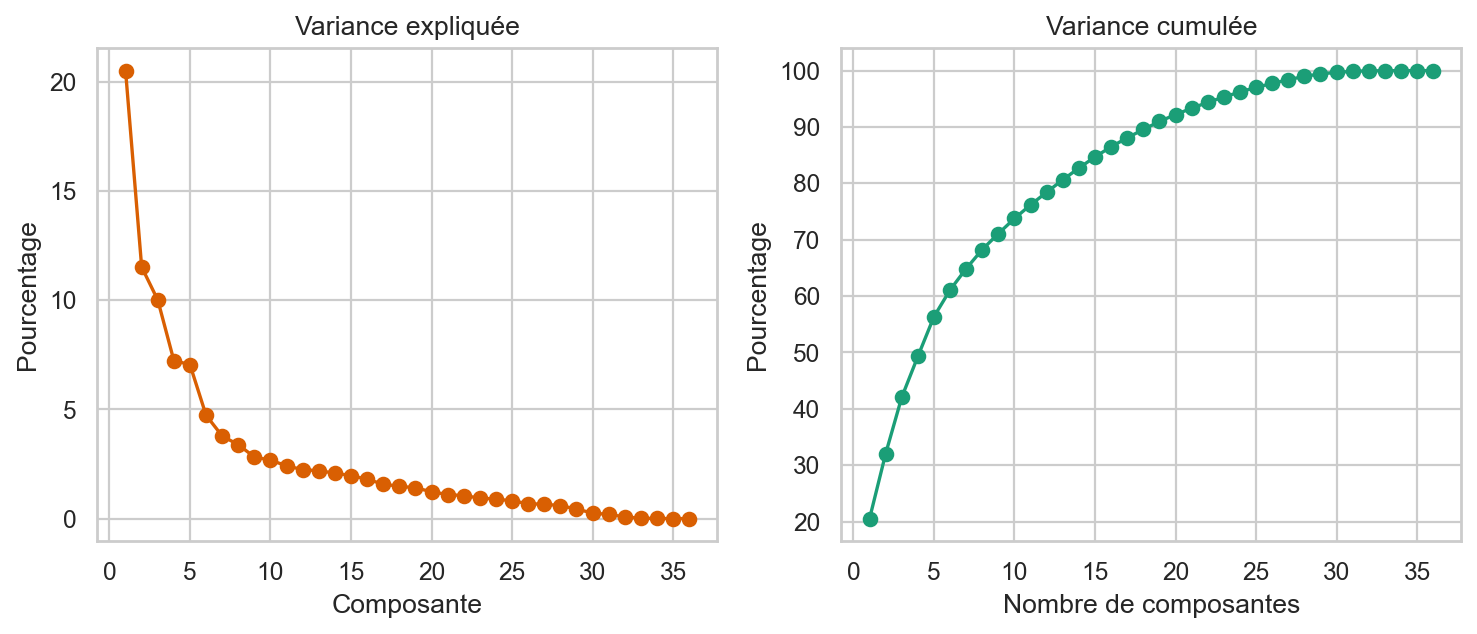
\includegraphics[width=0.9\textwidth]{figures_rapport/variance_acp.png}
    \caption{Variance expliquée par les composantes et variance cumulée.}
    \label{fig:variance}
\end{figure}

\subsection{Interprétation des profils}

Dans le cercle des corrélations, les variables proches sont positivement associées. Les variables orientées dans des directions opposées sont associées négativement. Une flèche longue et éloignée de l'origine contribue davantage à la construction du plan PC1--PC2.

Dans la projection des produits, deux produits proches dans le plan factoriel ont des profils nutritionnels comparables selon les variables retenues. Les produits situés aux extrêmes des axes correspondent à des profils plus atypiques. Ces extrêmes ne sont pas nécessairement des erreurs : ils peuvent représenter des produits particulièrement riches en énergie, en lipides, en minéraux ou en vitamines.

\begin{figure}[H]
    \centering
    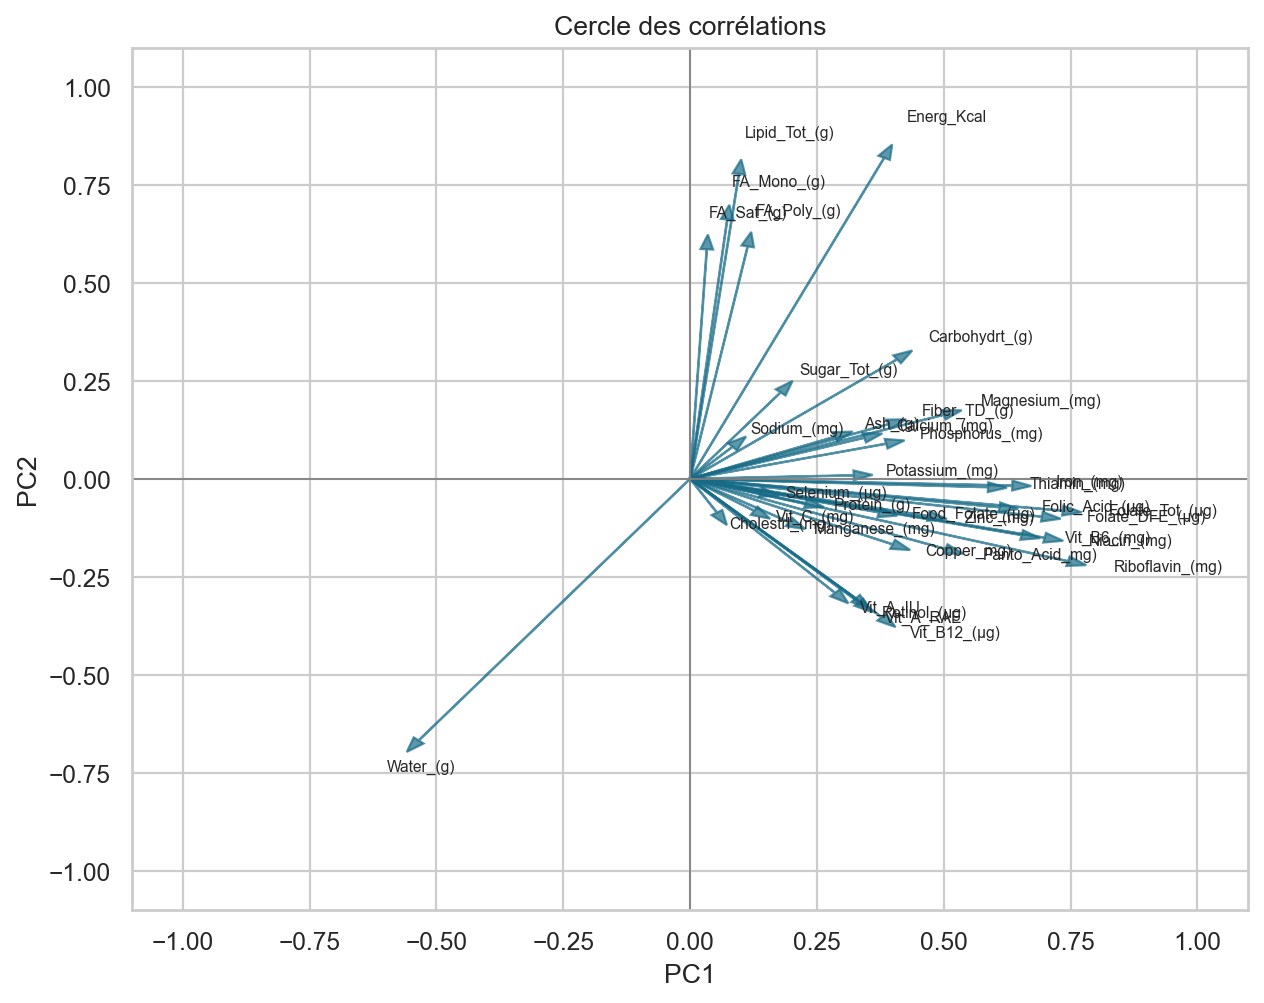
\includegraphics[width=0.86\textwidth]{figures_rapport/cercle_correlations.png}
    \caption{Cercle des corrélations sur les deux premiers axes.}
    \label{fig:cercle}
\end{figure}

\begin{figure}[H]
    \centering
    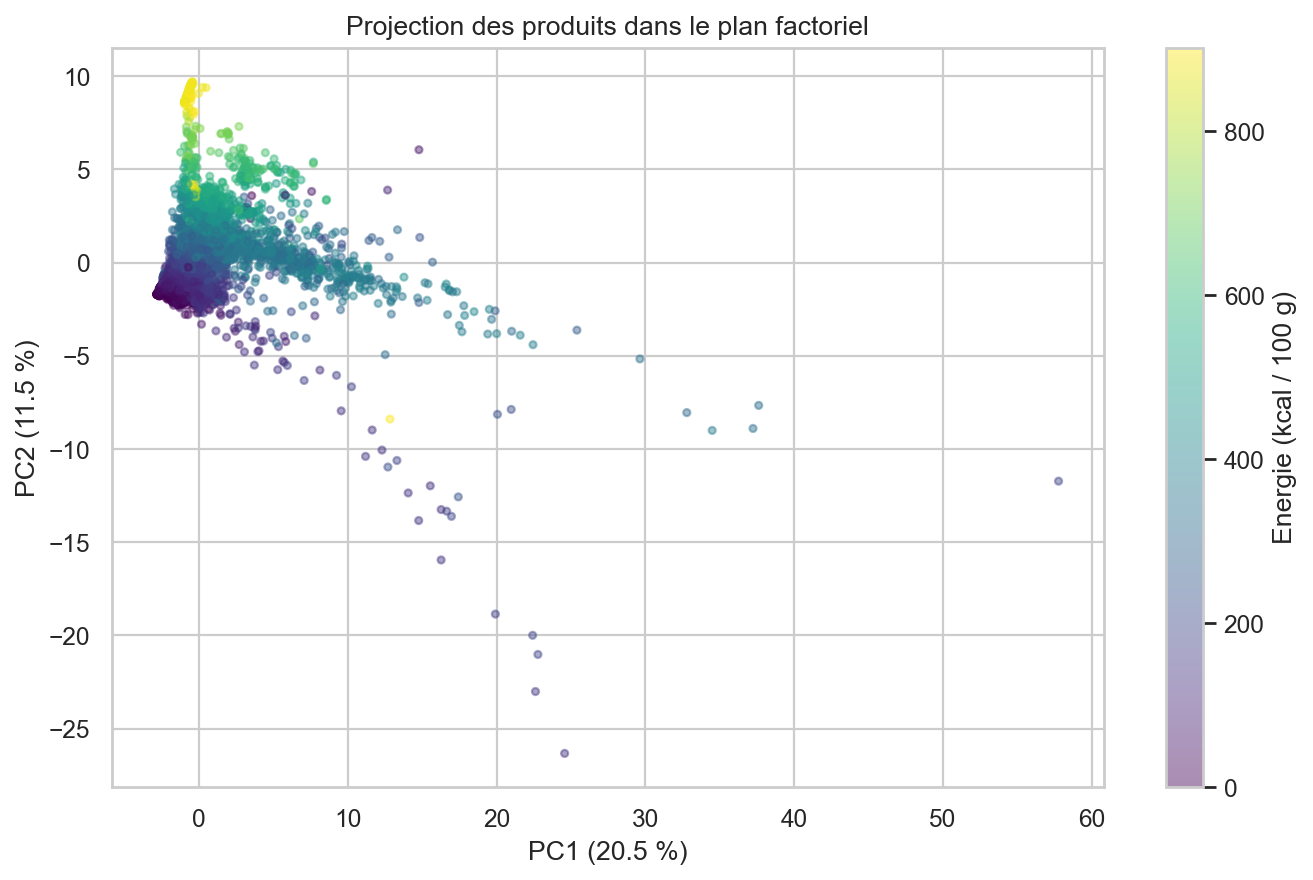
\includegraphics[width=0.88\textwidth]{figures_rapport/projection_produits.png}
    \caption{Projection des produits dans le plan factoriel, colorée par l'énergie.}
    \label{fig:projection}
\end{figure}

\section{Lecture des visualisations}

Les figures intégrées permettent de suivre l'analyse sans outil complémentaire. Elles montrent successivement :
\begin{enumerate}
    \item compréhension de la structure de la base ;
    \item qualité des données et statistiques descriptives ;
    \item matrice de corrélation et associations les plus fortes ;
    \item ACP, cercle des corrélations et projection des produits.
\end{enumerate}

La figure~\ref{fig:missing} documente la qualité des données. La figure~\ref{fig:distributions} met en évidence les dispersions et les asymétries. La figure~\ref{fig:correlations} permet de repérer les associations. Enfin, les figures~\ref{fig:variance}, \ref{fig:cercle} et \ref{fig:projection} résument l'ACP et les profils des produits.

\medskip
Une version interactive reste disponible en complément :\\
\noindent\textbf{Lien de démonstration :}\\
\url{https://usda-nutrition-app-9awedg4cm2qbog5la5j8ci.streamlit.app/}

\section{Limites et améliorations possibles}

\begin{itemize}
    \item La base contient des valeurs manquantes, et l'imputation par médiane peut réduire la variabilité observée.
    \item Les noms des produits ne constituent pas une variable catégorielle structurée ; une analyse par groupes alimentaires nécessiterait un dictionnaire complémentaire.
    \item Les corrélations étudiées sont linéaires et ne détectent pas toutes les relations non linéaires.
    \item Les deux premiers axes ne représentent que 32,04\% de la variance ; l'interprétation doit donc rester descriptive.
\end{itemize}

Des prolongements possibles sont une classification des produits dans l'espace factoriel, une analyse par familles alimentaires et une comparaison avec les recommandations nutritionnelles.

\section{Conclusion}

Cette étude met en évidence une forte diversité nutritionnelle entre les produits USDA. Plusieurs variables sont fortement associées, notamment les indicateurs proches de définition pour les vitamines et les folates. L'ACP permet de résumer les profils et de visualiser les produits similaires ou atypiques, même si les deux premiers axes ne capturent qu'une partie de l'information totale.

Le notebook et l'application Streamlit rendent l'analyse reproductible et interactive. Le code source est disponible sur GitHub :
\url{https://github.com/DALINGUESSAN/usda-nutrition-streamlit}.

\end{document}